\documentclass[diploma]{nanolab2015}

\begin{document}
\begin{titlepage}
\begin{center}
    \large
    ФЕДЕРАЛЬНОЕ ГОСУДАРСТВЕННОЕ БЮДЖЕТНОЕ ОБРАЗОВАТЕЛЬНОЕ УЧРЕЖДЕНИЕ ВЫСШЕГО ОБРАЗОВАНИЯ «МОСКОВСКИЙ ГОСУДАРСТВЕННЫЙ УНИВЕРСИТЕТ ИМЕНИ М.В.ЛОМОНОСОВА»
     
    \textbf{Физический факультет}\\
    \vspace{4cm}
    \textsc{\Large Отчет по практическому заданию №1}\\[5mm]
    {\LARGE Численные методы в физике.}
\end{center}
\vspace{7cm}
\null
\begin{flushright}
\normalsize студента 427 группы
\\Иванова Ивана Ивановича
\end{flushright}
\vfill
\begin{center}
\textbf{Москва - 2022}
\end{center}
\end{titlepage}


\section{Постановка задачи.}

Выполнить дискретное комплексное преобразование Фурье используя одну из библиотечных программ для БПФ при $N=16$ следующего сигнала:

\noindent $0.349469$, $1.106038$, $0.623345$, $-0.945356$, $-1.371444$, $-0.109880$, \
$1.045291$, $0.803699$, $-0.448111$, $-1.371336$, $-0.598131$, $0.927789$, \
$1.403043$, $0.102628$, $-1.132961$, $-0.793362$.

Используя полученные гармоники,  выполнить  обратное  преобразование  Фурье  и  сравнить  его с  исходными отсчётами. Также необходимо построить графики исходных отсчетов и спектральной плотности мощности.

\section{Используемый пакет для БПФ.}

Для решения поставленной задачи использовались функции Fourier и InverseFourier из Wolfram Mathematica. Опишу некоторые особенности используемых функций.

Первое, что необходимо учесть - тот факт, что в программе используется отличное от лекционного материала определение прямого и обратного преобразования Фурье. Этот факт можно исправить с помощью функции FourierParametrs(a,b), с помощью которой можно поменять параметры a и b:

$$U(k) = \frac{1}{N^{(1-a)/2}} \sum_{j=0}^{N-1} u(j) e^{\frac{ 2\Pi i b j k}{N}}$$

$$u(j) = \frac{1}{N^{(1+a)/2}} \sum_{k=0}^{N-1} U(k) e^{\frac{- 2\Pi i b j k}{N}}$$

Чтобы получить желаемый вид дискретного преобразования Фурье, необходимо положить $a = -1$ и $b = -1$, тогда получим следующий вид преобразования:

$$U(k) = \frac{1}{N} \sum_{j=0}^{N-1} u(j) e^{\frac{- 2\Pi i j k}{N}}$$

$$u(j) = \sum_{k=0}^{N-1} U(k) e^{\frac{2\Pi i j k}{N}}$$

Также, так как в данной задаче число N отсчётов сигнала является является степенью числа 2, Wolfram воспользуется этим фактом для ускорения расчёта дискретного преобразований Фурье (БПФ). Также данный алгоритм использует меньшее количество памяти. Также важно учитывать, что гармоника с нулевой частотой появляется на первой позиции результирующем списке.

 \section{Программа.}
На рисунке \ref{pic1} представлен код программы написанный в Wolfram Mathematica. Данная программа реализует прямое и обратное преобразование Фурье с помощью описанных выше функций, также здесь вычисляется спектральная плотность мощности сигнала и строится её спектр.

\begin{figure}[h!]
\centering
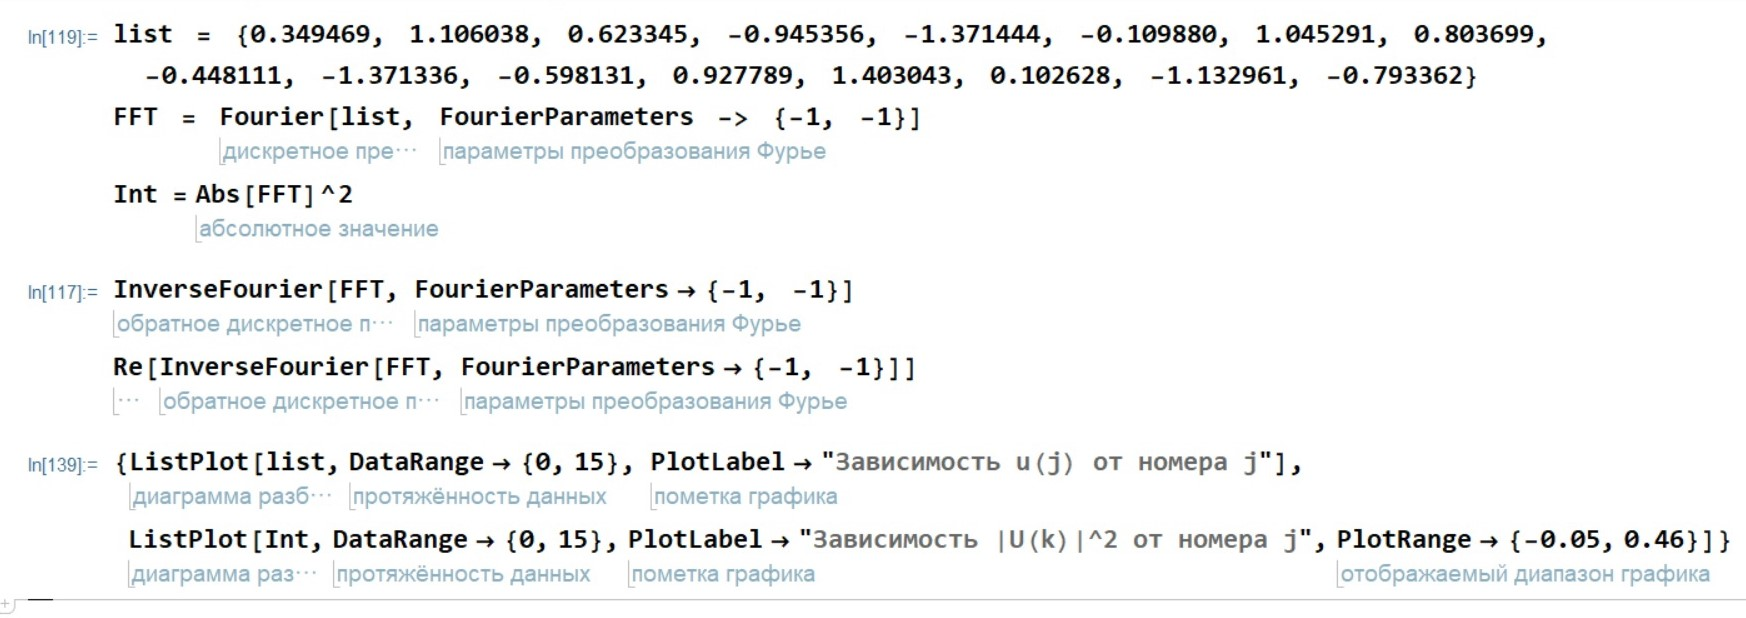
\includegraphics[scale=0.38]{prog.jpg}
\caption{\label{pic1}Код программы.}
\end{figure}
 
  \section{Результаты.} 
  Ниже приведена таблица значений $U(k)$ гармоник после дискретного преобразования Фурье исходного сигнала.
  
 \vspace{0.5 cm}
  \begin{tabular}{|c|c|}
  \hline 
  k & U(k) \\ 
  \hline 
  0 & -0.0255799 + 0 i \\ 
  \hline 
  1 & 0.0186776 + 0.0461369 i \\ 
  \hline 
  2 & -0.018311 + 0.00558207 i \\ 
  \hline 
  3 &  0.209077 -  0.608806 i \\ 
  \hline 
  4 &  -0.000286688 + 0.0165825 i \\ 
  \hline 
  5 &  -0.0248117 + 0.0385016 i \\ 
  \hline 
  6 & 0.00203087 + 0.0196926 i \\ 
  \hline 
  7 &  -0.00354798 - 0.000177683 i \\ 
  \hline 
  8 & 0.00939256 + 0 i \\ 
  \hline 
  9 & -0.00354798 + 0.000177683 i \\ 
  \hline 
  10 & 0.00203087 - 0.0196926 i \\ 
  \hline 
  11 & -0.0248117 - 0.0385016 i \\ 
  \hline 
  12 & -0.000286688 - 0.0165825 i \\ 
  \hline 
  13 & 0.209077 + 0.608806 i \\ 
  \hline 
  14 & -0.018311 - 0.00558207 i \\ 
  \hline 
  15 &  0.0186776 - 0.0461369 i \\ 
  \hline 
  \end{tabular} 
  
 \vspace{0.5 cm} 
  Также было произведено обратное преобразование Фурье и полученные значения немного отличаются от исходных значений:
  
  \begin{tabular}{|c|c|c|}
  \hline 
  j & u(j) исходное & u(j) восстановленное \\ 
  \hline 
  0 & 0.349469 & 0.349469 + 0 i\\ 
  \hline 
  1 & 1.10604 & $1.10604 + 2.36362*10^{-18} i$ \\ 
  \hline 
  2 &  0.623345 & $0.623345 + 0 i$ \\ 
  \hline 
  3 & -0.945356 & $-0.945356 + 5.57073*10^{-17} i$ \\ 
  \hline 
  4 &  -1.37144 & $-1.37144 + 0 i$ \\ 
  \hline 
  5 & -0.10988 & $-0.10988 - 1.13386*10^{-16} i$ \\ 
  \hline 
  6 &  1.04529 & $1.04529 + 0 i$ \\ 
  \hline 
  7 & 0.803699  &  $0.803699 - 5.57073*10^{-17} i$ \\ 
  \hline 
  8 & -0.448111  &  $-0.448111 + 0 i$ \\ 
  \hline 
  9 & -1.37134  &  $-1.37134 + 2.36362*10^{-18} i$ \\ 
  \hline 
  10 & -0.598131 &  $-0.598131 + 0 i$ \\ 
  \hline 
  11 &  0.927789 &  $0.927789 - 5.5315*10^{-17} i$ \\ 
  \hline 
  12 & 1.40304 & $1.40304 + 0 i$ \\ 
  \hline 
  13 & 0.102628 & $0.102628 + 1.08659*10^{-16} i$ \\ 
  \hline 
  14 & -1.13296 & $-1.13296 + 0 i$ \\ 
  \hline 
  15 & -0.793362 & $-0.793362 + 5.5315*10^{-17} i$  \\ 
  \hline 
  \end{tabular} 
  
  \vspace{0.5 cm}
  Из таблицы видно, что действительные части равны, а мнимые равны в пределах "машинной точности" вычислений. Полученный ответ можно записать в более красивом виде, используя, например, встроенную функцию Re, которая вернет список действительных частей исходного списка. Аналогичный ответ можно получить, если округлить исходный список, например, до 12 знака.
  
\begin{figure}[h!]
\centering
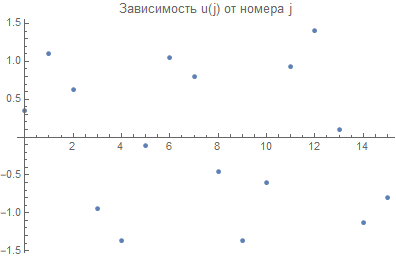
\includegraphics[scale=1.1]{1.png}
\caption{\label{pic2}Зависимость исходных отсчётов $u(j)$ от числа $j$.}
\end{figure}

\begin{figure}[h!]
\centering
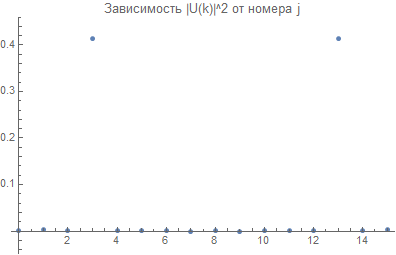
\includegraphics[scale=1.1]{2.png}
\caption{\label{pic3}Зависимость спектральной плотности мощности от номера гармоники $k$.}
\end{figure}

На рисунке \ref{pic2} изображёны исходные отсчёты сигнала, а на рисунке \ref{pic3} изображена зависимость спектральной плотности мощности от номера гармоники $k$. Из последней зависимости видно, что наибольший вклад в спектр вносят 3 и 13 гармоники, абсолютное значение которых равно $0.414357$.
\end{document}
